\section{Predikaatlogica}

\begin{answer} % 5.1
Welke van de volgende uitdrukkingen zijn formules en welke niet? Indien niet een formule, geef dan aan waarom. Indien het wel een formule is, geef aan wat de formule uitdrukt.
\begin{enumerate}[label=\roman*.]
\item $\exists x\forall y\;x=y$ \\
antwoord: Een syntactisch correcte formule. Er is een x waarvoor geldt dat hij gelijk is aan alle y. 
\item $\forall x\;x\geq y\rightarrow\exists z\; y=z$ \\
antwoord: Een syntactisch correcte formule. Als voor alle x geldt dat x groter of gelijk is aan y, dan is er een z die gelijk is aan y.
\item $\forall x\wedge\exists z\;R(x,z)$ \\
antwoord: Een syntactisch incorrecte formule. Een $\land$ tussen twee kwantoren is niet zinnig en mag niet van de syntax. 
\item $\forall x\;x\wedge\exists z\;z>y$ \\
antwoord: Een syntactisch incorrecte formule. x is een object en heeft geen waarheidswaarde los zonder een predikaat.
\item $\forall \forall y\exists z(x>y\vee y>z)$ \\ 
antwoord: Een syntactisch incorrecte formule. Twee keer $\forall$ achterelkaar mag niet van de syntax.
\end{enumerate}
\end{answer}

\begin{answer} % 5.2
Gegeven is een verzameling $V$ waarop een kleiner-of-gelijk relatie $\leq$ is gedefinieerd. Geef de volgende uitspraken weer in predikaatlogische formules met als predikaatsymboolen alleen $V$ en $\leq$.
\begin{enumerate}[label=\roman*.]
%a:
\item Er is een kleinste element in $V$. \\
antwoord: $\exists x \forall y (V(x) \land V(y) \land x \leq y)$
%b:
\item Er is geen grootste element in $V$. \\
antwoord: $\neg (\exists x \forall y (V(x) \land V(y) \land y \leq x))$ 
%c:
\item Er is een maximaal element in $V$ (dat wil zeggen: een element dat niet kleiner is dan enig ander element).\\
antwoord: $\exists x \forall y (V(x) \land V(y) \land y \leq x)$
\end{enumerate}
\end{answer}

\begin{answer} % 5.3
Geef in de volgende formules het bereik aan van $\forall y$, en geef aan welke variabelen vrij en gebonden zijn. (Uitdrukkingen als $y+z$ en $x+y$ zijn zoals gezegd eveneens termen, maar anders dan constanten en variabelen samengestelde termen).
\begin{enumerate}[label=\roman*.]
    % a:
    \item $\forall x\forall y\exists z\;y+z=x$ \\
    antwoord:  Alle variabelen zijn gebonden. Bereik van $\forall$y is onderstreept: \\
    $\forall x\forall y \underline{\exists z\;y+z=x}$.
    % b:
    \item $\forall y\exists z\;y+z=x$ \\ 
    antwoord: De variabelen y en z zijn gebonden. De variabele x is ongebonden. bereik van $\forall$y is onderstreept: \\
    $\forall y \underline{\exists z\;y+z=x}$
    % c:
    \item $\forall y\exists z\;y<z\wedge y>y$\\
    antwoord: De variabelen z en y zijn gebonden. De variabele y is ook voor een deel ongebonden. Het bereik van $\forall$y is onderstreept: \\
    $\forall y \underline{\exists z\;y<z}\wedge y>y$
    \item $P(y)\rightarrow\forall y\exists z\;y<z$ \\ 
    antwoord: De variabelen y en z zijn gebonden. De variabele y is ook voor een gedeelte ongebonden. Het bereik van $\forall$y is onderstreept: \\
    $P(y)\rightarrow\forall y \underline{\exists z\;y<z}$
\end{enumerate}
\end{answer}

\begin{answer} % 5.4
Maak gebruik van de afkortingen:

\begin{tabular}{lcl}
$M(x)$&:&$x$ is een man\\
$V(x)$&:&$x$ is een vrouw\\
$J(x,y)$&:&$x$ is jonger dan $y$\\
$K(x,y)$&:&$x$ is een kind van $y$\\
$G(x,y)$&:&$x$ en $y$ zijn met elkaar getrouwd
\end{tabular}\\
Schrijf, gebruik makend van bovenstaande afkortingen, met als universum de verzameling van alle mensen, in predikaatlogica:
\begin{enumerate}[label=\arabic*.]
    % a:
    \item Iedereen heeft een vader. \\
    antwoord: $\forall x \exists y (M(y) \land K(x, y))$
    % b:
    \item Iedereen is jonger dan zijn moeder. \\
    antwoord: $\forall x \exists y ((V(y) \land K(x, y)) \rightarrow J(x,y)) $
    \item Er is een man met een schoondochter die ouder is dan hij. \\
    antwoord: $\exists x \exists y \exists z(M(x)\land K(y,x) \land G(y,z) \land V(z) \land J(x,z))$
    \item $x$ is een grootvader van $y$. \\
    antwoord:$\exists z (K(y,z) \land K(z,x))$
    \item $x$ is een zuster van $y$.\\
    antwoord: $\exists z (V(x) \land K(x,z) \land K(y,z))$
    \item $x$ is een oom van $y$ van moeders kant. \\
    antwoord: $\exists z \exists w (K(y, z) \land V(z) \land K(z, w) \land K(x, w) \land M(x))$
\end{enumerate}
\end{answer}

\begin{answer} % 5.5
Gebruik de notatie $K(x,y)$ voor: $x$ is een kind van $y$. Schrijf in predikaatlogische notatie: $x$ heeft precies \'e\'en kind. \\
antwoord: $\exists y(K(y,x) \land \forall z (z = y \lor \neg K(z,x))) $
\end{answer}

\begin{answer} % 5.6
Als universum kiezen we de verzameling der re\"ele getallen. \\
Schrijf de volgende formules op in gewoon Nederlands, en ga na of ze waar zijn:
\begin{enumerate}[label=\arabic*.]
    \item $\forall x\exists y(x+y=3)$\\
    antwoord: Voor alle reële getallen geldt dat er een reëel getal is waarbij de som van die getallen gelijk is aan 3. \\
    Dit is waar. 
    \item $\exists x\forall y(x+y=3)$ \\
    antwoord: Er is minimaal één reëel getal waarvoor geldt dat je elk mogelijk reëel getal erbij kan optellen en dat je dan op 3 uitkomt. \\
    Dit is niet waar.
    \item $\exists x\exists y(x+y=3)$ \\
    Er is een reëel getal waarvoor geldt dat er een reëel getal is waarbij de som van beide getallen gelijk is aan 3. \\
    Dit is waar.
    \item $\forall x\forall y(x+y=3)$
    Voor alle reële getallen geldt dat er elk reëel getal bij op kan tellen en dat de uitkomst dan 3 is. \\
    Dit is niet waar.
\end{enumerate}
\end{answer}

\begin{answer} % 5.7
We bekijken de propositie
$$\forall x\forall t(P(x,t)\rightarrow\exists x(Q(x,t)\wedge\forall t(R(x,t))))$$
waarin $P(x,t)$, $Q(x,t)$ en $R(x,t)$ predikaten zijn.
\begin{enumerate}[label=\arabic*.]
    \item Geef voor elke voorkomende variabele met een pijl aan door welke kwantor hij wordt gebonden.\\
    Antwoord:
    \begin{center}
    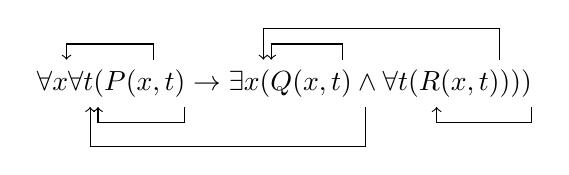
\begin{tikzpicture}
    \node[anchor=south west] at (0,0) {$\forall x\forall t(P(x,t)\rightarrow\exists x(Q(x,t)\wedge\forall t(R(x,t))))$};
    \draw[->] (1.6,.6) -- (1.6,.8) -- (.5, .8) -- (.5, .6); 
    \draw[->] (2,0) -- (2,-.2) -- (.9,-.2) -- (.9,0);
    \draw[->] (4,.6) -- (4,.8) -- (3.1,.8) -- (3.1,.6);
    \draw[->] (4.3,0) -- (4.3,-.5) -- (.8,-.5) --(.8,0);
    \draw[->] (6,.6) -- (6,1) -- (3,1) -- (3,.6);
    \draw[->] (6.4,0) -- (6.4,-.2) -- (5.2,-.2) -- (5.2,0);
    \end{tikzpicture}
    \end{center}
    \item Zorg er door hernoemen van variabelen voor dat eenzelfde letter niet in verschillende scopes optreedt.\\
    Antwoord:
    $$\forall x_1\forall t_1(P(x_1,t_1)\rightarrow\exists x_2(Q(x_2,t_1)\wedge\forall t_2(R(x_2,t_2))))$$
\end{enumerate}
\end{answer}

\begin{answer} % 5.8
Maak gebruik van de volgende afkortingen:
\begin{itemize}
  \item $G(x,y)$ betekent `$x$ is getrouwd met $y$';
  \item $K(x, y, z)$ betekent `$z$ is kind van $x$ en $y$'.
\end{itemize}
\begin{enumerate}[label=\arabic*.]
    \item Schrijf als predikaatlogische formule: `alle kinderen hebben twee ouders'. \\
    antwoord: $\forall x \exists y \exists z(K(x,y,z) \land y \neq z)$
    \item Idem: `niet alle getrouwde mensen hebben kinderen, maar alle kinderen hebben getrouwde ouders'.\\
    antwoord:\\[2pt] $\neg\Bigl[\forall x\forall y(G(x,y)\rightarrow\exists z\;K(x,y,z)\Bigr]\wedge
    \Bigl[\forall u\exists v\exists w(K(v,w,u)\rightarrow G(v,w)\Bigr]$
    \item Schrijf in goed Nederlands (gebruik geen variabelen):\\
    $\forall z\bigl[(\exists x\exists y(K(x, y, z)\wedge\neg G(x,y))\rightarrow\bigr.$\\
    \null\hfill$\bigl.(\exists u\exists v(K(u,v,z)\rightarrow\forall t(K(u,v,t)\rightarrow t=z))))\bigr]$\\
    antwoord: `Voor iedereen die een kind is van ongetrouwde ouders geldt dat zij enig kind zijn.'
\end{enumerate}
\end{answer}
